\chapter{Quality Attributes and Measurement}
\section{Quality Attributes}
Developers prioritize attributes and design systems that meet their needs.\\
\subsection{Availability}
Ability to avoid completely or recover quickly from failures. Redundancy.
\subsection{Performance}
Ability to meet timing or throughput requirements. The system needs to be able to respond quickly to events.
\subsection{Scalability}
Ability to scale the system performance to meet increased load. The system needs to be able to handle more concurrent requests.
\subsection{Security}
Ability to protect information. The system needs to be able to protect information from unauthorized access while still allowing authorized access.

\section{Scalability}
\subsection{When is software ready for release?}
It's ready for release when it's \textbf{dependable}. This means it needs to be correct, reliable, safe, and robust.
\subsubsection{Correctness}
A program is correct if it is always consistent with its specification. This depends on quality and detail of requirements, it's really easy to build a correct program with a weak specification, but if it's too detailed it becomes impossible to prove your program is completely correct.\\
\\
More often than not, correctness is something we aim for, not prove.
\subsubsection{Reliability}
A statistical approximation of correctness, the probability that the program will perform correctly during a given period of time under a given set of conditions. We test reliability by running the program as different types of user profiles, and mainly focuses on reliability for our target audience.

\subsubsection{Dependence on specifications}
Correctness and reliability are dependent on the quality and strength of the specification. The more detailed the specification, the more likely the program is to be correct and reliable in the real world.\\
\\
Correctness and reliability doesn't consider the severity of different crashes and bugs, a program that crashes once a year is more reliable than one that crashes once a day while in the real world it might be better with a daily crash than leaking all personal data once a year.\\

\subsubsection{Safety}
Safety is the ability to avoid hazards. We specify a set of undesirable situations, hazards, and prove that our program avoids them.\\

\subsubsection{Robustness}
Software that is correct may fail when our design assumptions are violated; \textit{how} it fails matters. Software that gracefully fails is robust, e.g. if we tries to save a program to a read-only disk, the program should tell us what wet wrong gracefully instead of crashing.\\
\\
Robustness cannot be proven, but is rather a goal to aspire to.

\subsection{Dependability}
We could have software that is reliable, but not correct, or correct but not safe, or robust but not safe. We need to consider all of these attributes when we talk about dependability.\\
\subsubsection{Measuring Dependability}
We need to establish criteria for when our system is dependable enough for release.\\
Correctness is too hard to prove conclusively for most programs.\\
Robustness and safety is important, but doesn't prove that our program functions correctly.\\
\textbf{Reliability is the basis for arguing dependability}, we can measure it, and we can demonstrate it through testing.

\section{Reliability}
Reliability is the probability of failure-fre operation for a specified time in a specified environment for a given purpose. This depends heavily on the system and user type.\\
\subsection{Improving reliability}
Reliability is improved when faults in our most frequently used parts are removed, this means that a program is more or less reliable for different users.
\subsection{Reliability is measurable}
Reliability can be defined and measured. We can specify requirements (both functional and non-functional) and measure how well our program meets them.
\subsection{How to measure reliability}
Hardware metrics often aren't suitable for software, since in hardware it can only hard crash and we can assume that the design of the hardware is correct.\\
\\
With software most of the failures are design failures, and when a system has failed the system is often still available.

\subsubsection{Availability}
Can the software carry out its given task when needed. Can the system avoid failures, and recover quickly from failures. Can the system beep working for other users when it has crashed for one?\\
\\
Availability is only a measurement of whether the system is available, not whether it's correct or reliable meaning incorrect computations or security isn't considered.\\
\\
Availability is also a standalone quality attribute. We can through design prevent, tolerate, remove, or forecast failures. We can keep our system partially available more easily than hardware.

\subsubsection{Probability of Failure on Demand (POFOD)}
Likelihood that a single request will result in failure. A POFOD of $0.001$ means that there is a 0.1\% chance that a single request will fail. This is used in situations where failure is unacceptable, e.g. a medical system.

\subsubsection{Rate of Occurrence of Fault (ROCOF)}
Frequency of occurence of unexpected behaviour. A ROCOF of $0.02$ means that we have 2 failure per 100 time units. Is appropriate when requests are made regularly, like a web server.

\subsubsection{Mean Time Between Failures (MTBF)}
Average time between failures. If we have a system that is used for long sessions, especially where users might only save their data once every few hours or so, it might be important to prevent crashes happening too often.
\subsection{Reliability Metrics}
\begin{itemize}
	\item Availability: $\frac{\text{Uptime}}{\text{Total time observed}}$
	\item POFOD: $\frac{\text{Failures}}{\text{Requests over period}}$
	\item ROCOF: $\frac{\text{Failures}}{\text{Time elapsed in target unit}}$
	\item MTBF: Average time between observed failures.
	\item MTTR: Average time to recover from failures.
\end{itemize}
It may be cheaper to accept some unreliability and pay for failure cost instead of trying to make the system more reliable. This depends on social/political factors.

\section{Performance}
The ability to meet timing or throughput requirements. This is the driving factor in software design, even though it is often at expense of other quality attributes. All systems have performance requirements, but they are often not specified. Bad performance leads to a decrease in users.
\subsection{Performance Measurements}
\begin{itemize}
	\item Latency
	      \subitem The time between arrival of stimulus and the systems response to it.
	\item Response Jitter
	      \subitem The allowable variation in latency.
	\item Throughput
	      \subitem Usually number of transactions per unit time.
	\item Deadlines in processing
	\item Number of events not processed
\end{itemize}
\subsubsection{Latency}
Time it takes to complete an interaction, how quickly the system responds to a user. We measure latency probabilistically, e.g. 95\% of requests are completed within 100ms.\\
\\
Another type of latency is the turnaround time, the time it takes to complete a larger task, e.g. With daily throughput of 850,000 requests, process should take < 4 hours, including writing to a database.

\subsubsection{Response Jitter}
Response time is non-deterministic, if we have an average latency of 5 seconds, we might have a latency of 2 minutes at a specific time, response jitter defines how large the maximum latency can be.

\subsubsection{Throughput}
The workload a given system can handle, usually measured in transactions per unit time. Since a larger throughput can lead to a longer service time, this can conflict with latency requirements.

\subsubsection{Deadlines}
Some special tasks must take place at a specific time.

\subsubsection{Missed events}
If our system is busy, we might need to ignore some events. This is usually a problem for real-time systems.

\section{Scalability}
The ability to process an increasing number of requests. There are two types of scalability:
\begin{itemize}
	\item Horizontal scalability
	      \subitem Adding more resources to the system, e.g. adding more servers to a web server farm.
	\item Vertical scalability
	      \subitem Adding more power to a single resource, e.g. adding more RAM to a single server.
\end{itemize}
How can we effectively utilize additional resources? This requires that additional resources:
\begin{itemize}
	\item Result in performance improvement
	\item Didn't require undue effort to add
	\item Did not disrupt operations
	\item \textbf{Must be designed to scale}
\end{itemize}

\section{Security}
Ability to protect data and information from unauthorized access while still providing access to authorized people and systems.\\
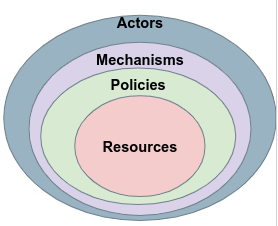
\includegraphics{lessons/images/security.png}\\
Processes allow owners of resources to control access. Actors are systems or users. Resources are sensitive elements, operations, and data of the system. Policies define legitimate access to resources.
\subsection{Security Characterization (CIA)}
Confidentiality, Integrity, and Availability.\\
Authentication, Nonrepudiation and Authorization are also important.\\
\subsection{Security Approaches}
We achieve security by detecting, resisting, reacting, and recovering from attacks. Data needs to be protected, both when in transit or when at rest.\\
\\
Security is a process, not a product. Nothing is completely secure or unsecure, and all systems will be compromised.  We need to be able to detect and recover from attacks as well as figure out who attacked.
\subsection{Assessing Security}
Measure of system's ability to protect data from unauthorized access while still providing service to authorized users. we need to assess how well system responds to attack. We can respond by e.g. logging, blocking, or shutting down the system.\\
\\
There isn't one single metric for measuring security, in some cases what data is more important, in some cases how much data was lost.

\section{Key points}
Dependability is one of the most improtant software characteristicts. Reliability depends on the pattern of usage of the software, different users will interact differently.\\
Reliability measured using ROCOF, POFOD, AVAILABILITY, MTBF, MTTR.\\
AVAIlability is the ability of the system to be available for use.
Performance is about management of resources in the face of demand to achieve acceptable timing
Scalability is the ability to “grow” the system to process an increasing number of requests
Security is the ability to protect data and information from unauthorized access
Security is not “measured”, but requires defining attacks and actions to prevent or reduce impact of risk, then assessing those actions